\chapter{Tworzenie edytorów graficznych na bazie metamodeli}

Aplikacje komputerowe wykorzystują elementy graficzne aby ułatwić i
przyśpieszyć użytkownikom pracę.
Dzieje się to z uwagi na fakt, że ludzie bardziej efektywnie przyswajają
informacje wizualne (obrazki, diagramy), niż
tekst~\cite{images-more-effective-article}.
W przypadku użytkownika
wpływającego na~zachowanie systemu w sposób wizualny (np.\ edytując diagram),
korzysta on wtedy z~edytora graficznego i modyfikuje pewien model
rzeczywistości reprezentowany przez program. Model ten zaprojektowany jest
przez twórcę aplikacji i jego struktura również może być~reprezentowana na
wiele sposobów. Jeżeli struktura modelu sama jest opisywana przez model (o
wyższym poziomie abstrakcji) to mówimy, że~ten model modelu to
\emph{metamodel}.

\section{Metamodelowanie}

\emph{Metamodelowanie} w kontekście wytwarzania oprogramowania to
technika polegająca
na~przygotowaniu abstrakcyjnego modelu (metamodelu) opisującego strukturę
modeli, które będą wykorzystywane w programie. Metamodel określa jakie są
dopuszczalne typy obiektów w~modelu, ich atrybuty, powiązania między nimi.
Definiuje składnię języka projektowania. Przedrostek \emph{meta} oznacza, że
poziom abstrakcji tego metamodelu jest wyższy niż poziom abstrakcji modelu,
który opisuje~\cite{from-requirements-to-java-in-a-snap}.

W rodzinie metamodeli~\cite{introduction-to-metamodels} przestrzenią o
najmniejszym poziomie abstrakcji jest
świat rzeczywisty (przestrzeń \emph{M0}). W programach komputerowych będzie on
reprezentowany przez model, który znajduje się w przestrzeni o wyższym poziomie
abstrakcji, \emph{M1}. Idąc dalej, modele będą oparte na metamodelach dla danej
dziedziny, które znajdują się w przestrzeni \emph{M2}. One~z~kolei są oparte na
meta--metamodelach % chktex 8
z przestrzeni \emph{M3}, które mają najwyższy poziom
abstrakcji w tej rodzinie. \emphgls{MOF}~\cite{mof-omg-specification} jest
przykładem meta--metamodelu. % chktex 8
Jest~zdefiniowany za pomocą samego siebie.

Wiele powszechnie znanych języków projektowania diagramów ma swoje metamodele
definiujące ich strukturę:

\begin{itemize}
	\item \emphgls{UML} ma swoją specyfikację~\cite{uml-omg-specification}
	      i metamodel opisany w języku \emphgls{MOF}.

	\item \emphgls{BPMN} (język do opisu procesów biznesowych) ma swój
	      metamodel~\cite{bpmn-omg-specification} również opisany w języku
	      \emphgls{MOF}.

	\item Istnieje artykuł proponujący metamodel dla
	      \emphgls{ERM}~\cite{entity-relationship-metamodel}.
	      Dla~przypomnienia,
	      \emphgls{ERM} pozwala przedstawić na diagramie encje bazy danych
	      i~powiązania
	      między nimi.
\end{itemize}

W metamodelu zdefiniowana jest składnia abstrakcyjna modelu, czyli struktura
jego elementów, oraz składnia konkretna, czyli jak one mają być reprezentowane,
na przykład na~diagramie.
Aby model był funkcjonalny oprócz jego struktury (składni języka projektowania)
należy zdefiniować i przestrzegać jego semantyki. To ona decyduje o tym jak
należy interpretować model, a także jakie sytuacje, pomimo bycia poprawnymi
strukturalnie, byłyby niewłaściwe z~punktu widzenia ich sensowności.

Przykładowo, w języku \emphgls{UML} z perspektywy struktury możliwe jest
utworzenie dwóch klas i dwóch połączeń kompozycji między nimi, co zostało
zademonstrowane na rysunku~\ref{rys:nieprawidlowy-model-uml}. Taki model jest
semantycznie niepoprawny, ponieważ relacja kompozycji oznacza, że jeden obiekt
jest zawarty w drugim obiekcie. Oznaczałoby to, że zarówno osoba
(\emph{Person}) jest zawarta w obiekcie samochodu (\emph{Car}) jako jego
właściciel, jak i samochody są zawarte w obiekcie właściciela.

\begin{figure}[!hb]
	\centering

	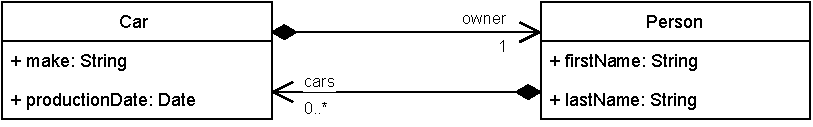
\includegraphics[width=0.95\linewidth]{./images/invalid-uml-example.pdf}
	\caption{Przykład modelu \emphgls{UML} nieprawidłowego
		semantycznie}\label{rys:nieprawidlowy-model-uml}
\end{figure}

Dopiero znając znaczenie relacji kompozycji można zauważyć ten błąd semantyczny
i~go~poprawić, na przykład jak na rysunku~\ref{rys:prawidlowy-model-uml}. Na
tym diagramie to osoba (\emph{Person}) jest obiektem nadrzędnym, który może
zawierać w sobie odniesienia do samochodów (\emph{Car}). Taki diagram jest
poprawny zarówno składniowo, jak i semantycznie.

\begin{figure}[!hb]
	\centering

	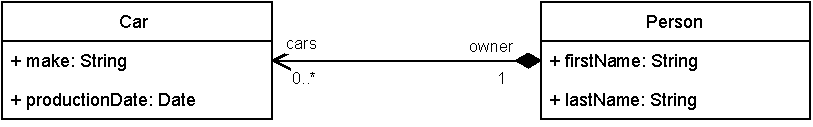
\includegraphics[width=0.95\linewidth]{./images/valid-uml-example.pdf}
	\caption{Przykład prawidłowego modelu
		\emphgls{UML}}\label{rys:prawidlowy-model-uml}
\end{figure}

\section{Edytory graficzne na podstawie metamodeli}

Metamodele mogą być zapisane w formacie, który jest przyjazny do odczytu
maszynowego. Oznacza to, że narzędzia będą mogły go odczytać, zinterpretować, a
także edytować. Sam~metamodel może mieć swój meta-metamodel, który zdefiniuje
jego strukturę.

Taki sformalizowany sposób przechowywania metamodelu ma wiele
korzyści. Przede wszystkim metamodel może być wtedy projektowany i edytowany w
narzędziu umożliwiającym robienie tego w najprostszy dla użytkownika sposób, na
przykład poprzez reprezentację metamodelu jako diagram. Ponadto, narzędzia mogą
wygenerować kod w konkretnym języku programowania. Zawierać on może klasy lub
inne mechanizmy przedstawienia modelu w tym języku programowania oraz może
wspierać operacje takie jak edycja, sprawdzenie poprawności składniowej
modelu.

Skoro znana jest struktura modelu, a więc wszystkie możliwe elementy i ich
połączenia, możliwe jest stworzenie edytora modeli, który będzie oparty na
metamodelu. Otrzymanie edytora diagramów dla danej dziedziny odbywa się dzięki
temu niskim nakładem czasowym --- wystarczy zdefiniować metamodel dziedziny, a
także zdefiniować wygląd elementów. Wymaga to mniejszej ilości czasu i
umiejętności w porównaniu z budową edytora diagramów korzystając z
edytorów diagramów ogólnego zastosowania.

\begin{figure}[!b]
	\centering

	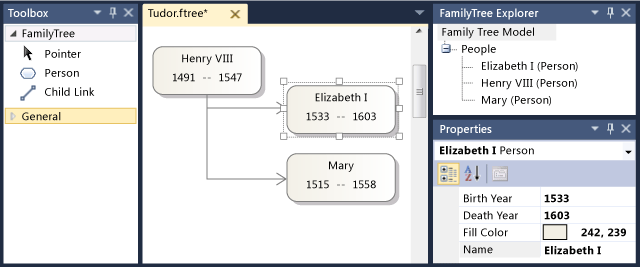
\includegraphics[width=0.95\linewidth]{./images/visual-studio-dsl-example.png}
	\caption{Edytowanie modelu w \emph{Visual Studio DSL
			Tools}}\label{rys:visual-studio-dsl-example}
\end{figure}

Przykładem zestawu narzędzi dostarczającego możliwości metamodelowania i
późniejszego generowania edytora graficznego dla modelu jest \emph{Visual
	Studio DSL Tools}~\cite{visual-studio-dsl-introduction} utworzone przez
firmę \emph{Microsoft}. Jest to zestaw
narzędzi do definiowania metamodelu, a następnie przygotowania rozszerzenia do
\emph{Visual Studio} w formacie \emphgls{VSIX}. Po jego zainstalowaniu
\emph{Visual Studio} nabiera możliwości graficznego edytowania modeli
bazujących na danym metamodelu. Edycja przykładowego modelu przedstawiona jest
na rysunku~\ref{rys:visual-studio-dsl-example}. Ponadto, tak przygotowany
edytor
może również generować klasy języka \emph{C\#} pozwalające na reprezentację
modelu, a
także jego serializację i deserializację. Dodatkową funkcjonalnością jest
również możliwość tworzenia plików na podstawie szablonów przygotowanych dla
metamodelu. W ten sposób można wygenerować na przykład tabelę w~języku
\emphgls{HTML} zawierającą wszystkie elementy konkretnego typu w modelu.

Innym narzędziem umożliwiającym przygotowanie edytora graficznego na podstawie
metamodelu jest \SiriusDesktop{}~\cite{sirius-desktop-homepage} rozwijany
przez firmę \Eclipse{}. Jest to rozszerzenie do~zintegrowanego środowiska
programistycznego (\emphgls{IDE}) \Eclipse{}. Pozwala ono na zaprojektowanie
metamodelu dla wybranej dziedziny używając technologii \emph{\acrfull{EMF}}.
Jest on wyrażony za pomocą
meta--metamodelu  % chktex 8
\Ecore{} (rozszerzenie \texttt{*.ecore}) i jest
zapisany w pliku \emphgls{XML}. Interfejs użytkownika programu \SiriusDesktop{}
widoczny jest na rysunku~\ref{rys:sirius-desktop-example-metamodel}. Po lewej
dostępne jest drzewo metaklas, na środku widać diagram struktury struktury
metamodelu, a po prawej stronie znajduje się przybornik z~narzędziami do
tworzenia elementów metamodelu. W \SiriusDesktop{}
można wygenerować 5 pakietów opisanych w kolejnych akapitach.

\begin{figure}[!ht]
	\centering

	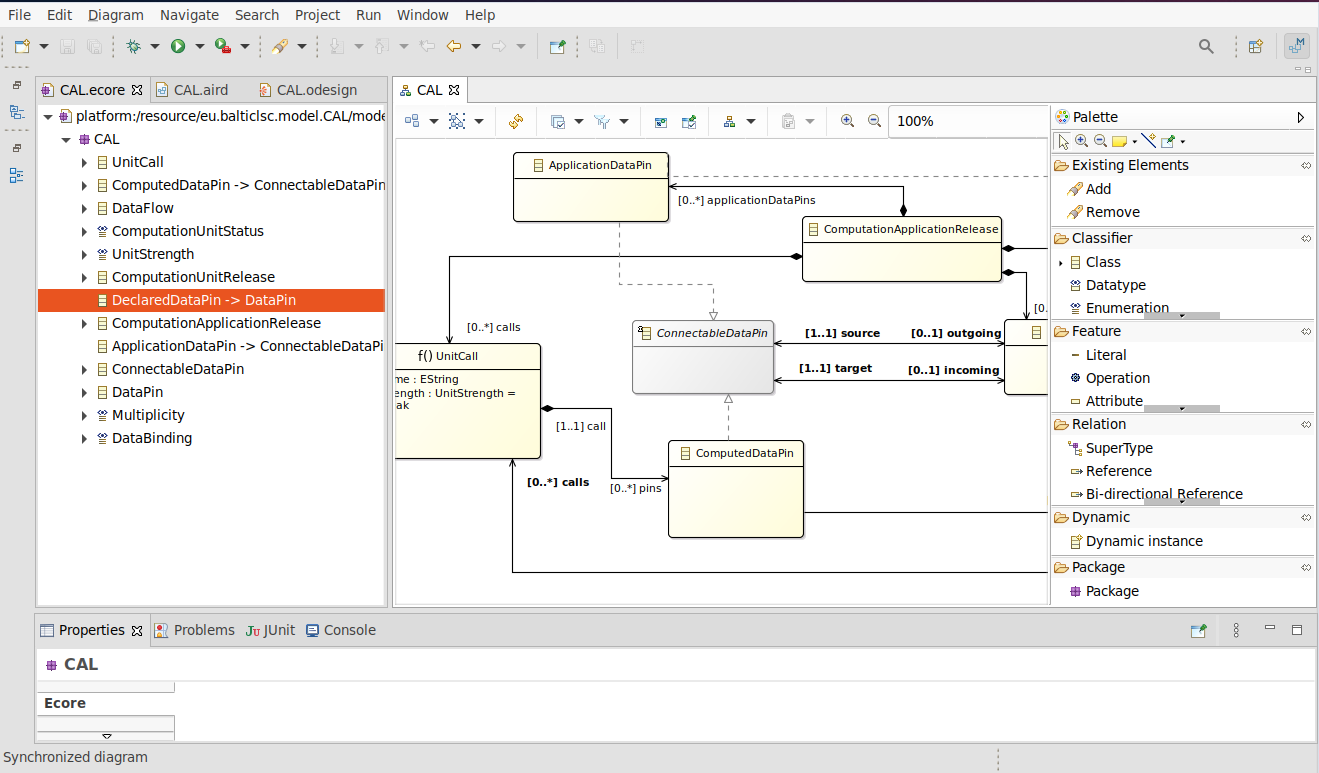
\includegraphics[width=0.95\linewidth]{./images/sirius-desktop-metamodel.png}
	\caption{Projektowanie metamodelu w \emph{Sirius
			Desktop}}\label{rys:sirius-desktop-example-metamodel}
\end{figure}

Pierwszym pakietem jest pakiet bazowy zawierający klasy umożliwiające
reprezentację modeli w
kodzie języka \Java{}, ich serializację i deserializację. Każdy obiekt
metamodelu
odpowiada klasie języka \Java{}. Klasy te zawierają mechanizmy powiadamiana o
zmianach (ang.~\emph{\selectlanguage{english}change detection}).
Możliwa jest modyfikacja kodu tych klas, co zmienia zachowanie
modelu.

Drugim z pakietów jest pakiet \texttt{.design} z plikiem o rozszerzeniu
\texttt{*.odesign} zawierający opis reprezentacji graficznych modelu. Każdy
model może mieć wiele reprezentacji graficznych z~różnymi poziomami
szczegółowości.
Możliwe reprezentacje graficzne to diagram klas, diagram
sekwencji, tabela, drzewo~\cite{dokumentacja-sirius-desktop}. Dla każdej
reprezentacji należy zdefiniować jak elementy modelu mają być wyświetlane.

Funkcjonalności ulepszające doświadczenia użytkownika z
korzystania z edytora zawierają także możliwość ustalenia styli warunkowych
(zmiany wyglądu elementu gdy spełnione zostaną ustalone warunki), zdefiniowanie
narzędzi pomagających w edycji diagramu (przykładowo okno dialogowe
wyświetlające formularz składający się z kilku kroków, który ostatecznie tworzy
kilka powiązanych ze sobą obiektów w modelu, albo narzędzie do kaskadowego
usuwania powiązanych elementów modelu), jak i możliwość opisania reguł
walidacji semantycznej, które będą uruchamiane po każdej zmianie i będą mogły
oznaczyć niepoprawne elementy modelu oraz zaproponować automatyczne ich
naprawienie.

Operacje wymagające wykonania dynamicznej logiki mogą być wprowadzone na 2
sposoby: poprzez napisanie kodu w języku \Java{} i udostępnienie go jako usługa
dostępna w~metamodelu, lub poprzez napisanie wyrażenia w języku
\emphgls{AQL}~\cite{dokumentacja-aql}.
Pozwala on~na~wybranie elementów z modelu (także podzbioru elementów
spełniających pewne kryteria), ich~atrybutów, oraz wykonanie operacji
logicznych na nich, na przykład ich~porównanie.

Trzecim pakietem jest pakiet \texttt{.edit}. Składa się on z klas
umożliwiających programatyczne odczytanie informacji o strukturze modelu ---
klasy zawierają opis właściwości obiektów modelu.

Czwartym pakietem jest pakiet \texttt{.editor}. Zawiera on definicję wtyczki do
środowiska \Eclipse{}, która dostarcza możliwości tworzenia i edycji
modeli. To właśnie ten pakiet umożliwia użycie wszystkich pozostałych pakietów
przez użytkownika i ostatecznie otrzymanie edytora graficznego. Edytor
diagramów dla przykładowego modelu został zaprezentowany na
rysunku~\ref{rys:sirius-desktop-example-model}.

\begin{figure}[!ht]
	\centering

	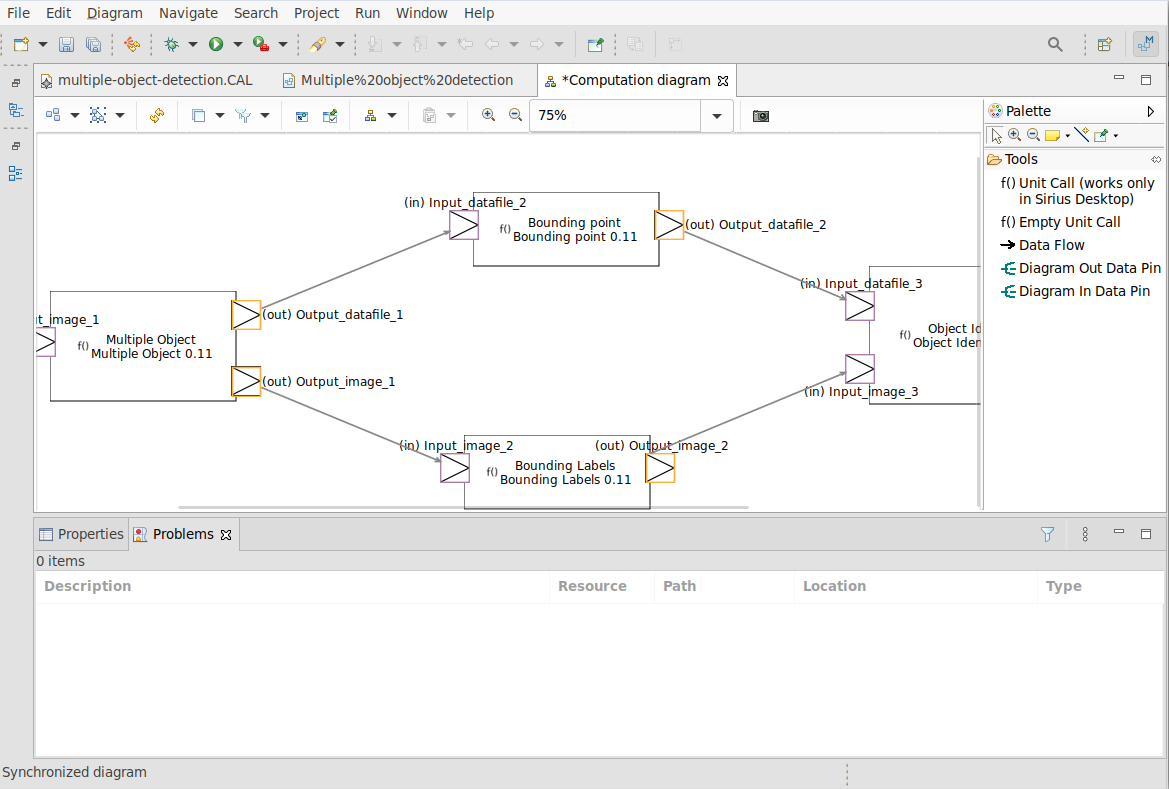
\includegraphics[width=0.95\linewidth]
	{./images/sirius-desktop-model-editor.png}
	\caption{Edycja przykładowego modelu w
		\SiriusDesktop{}}\label{rys:sirius-desktop-example-model}
\end{figure}

Piątym pakietem jest pakiet \texttt{.tests}. Można w nim tworzyć testy
zachowania metamodelu korzystając z środowiska uruchomieniowego do testów
\JUnit{}. Testy te przydają się~gdy~domyślne zachowanie modelu zostanie
zmodyfikowane poprzez edycję klas bazowych modelu w~głównym pakiecie projektu.

Edytor graficzny otrzymany dzięki pakietowi \texttt{.editor} jest wtyczką do
środowiska \Eclipse{}, które jest aplikacją systemową wymagającą instalacji
w systemie użytkownika zanim będzie on~mógł przeglądać i edytować modele.
Od 2018 roku~\cite{sirius-components-repo-first-commit} firma \Eclipse{}
pracuje nad~rozwiązaniem \SiriusWeb{}~\cite{sirius-web-github}, którego
celem jest przeniesienie edytora
graficznego dotychczas dostępnego w aplikacji natywnej do przeglądarki
internetowej. Interfejs użytkownika tego projektu jest widoczny na
rysunku~\ref{rys:sirius-web-ui}.

\begin{figure}[!ht]
	\centering

	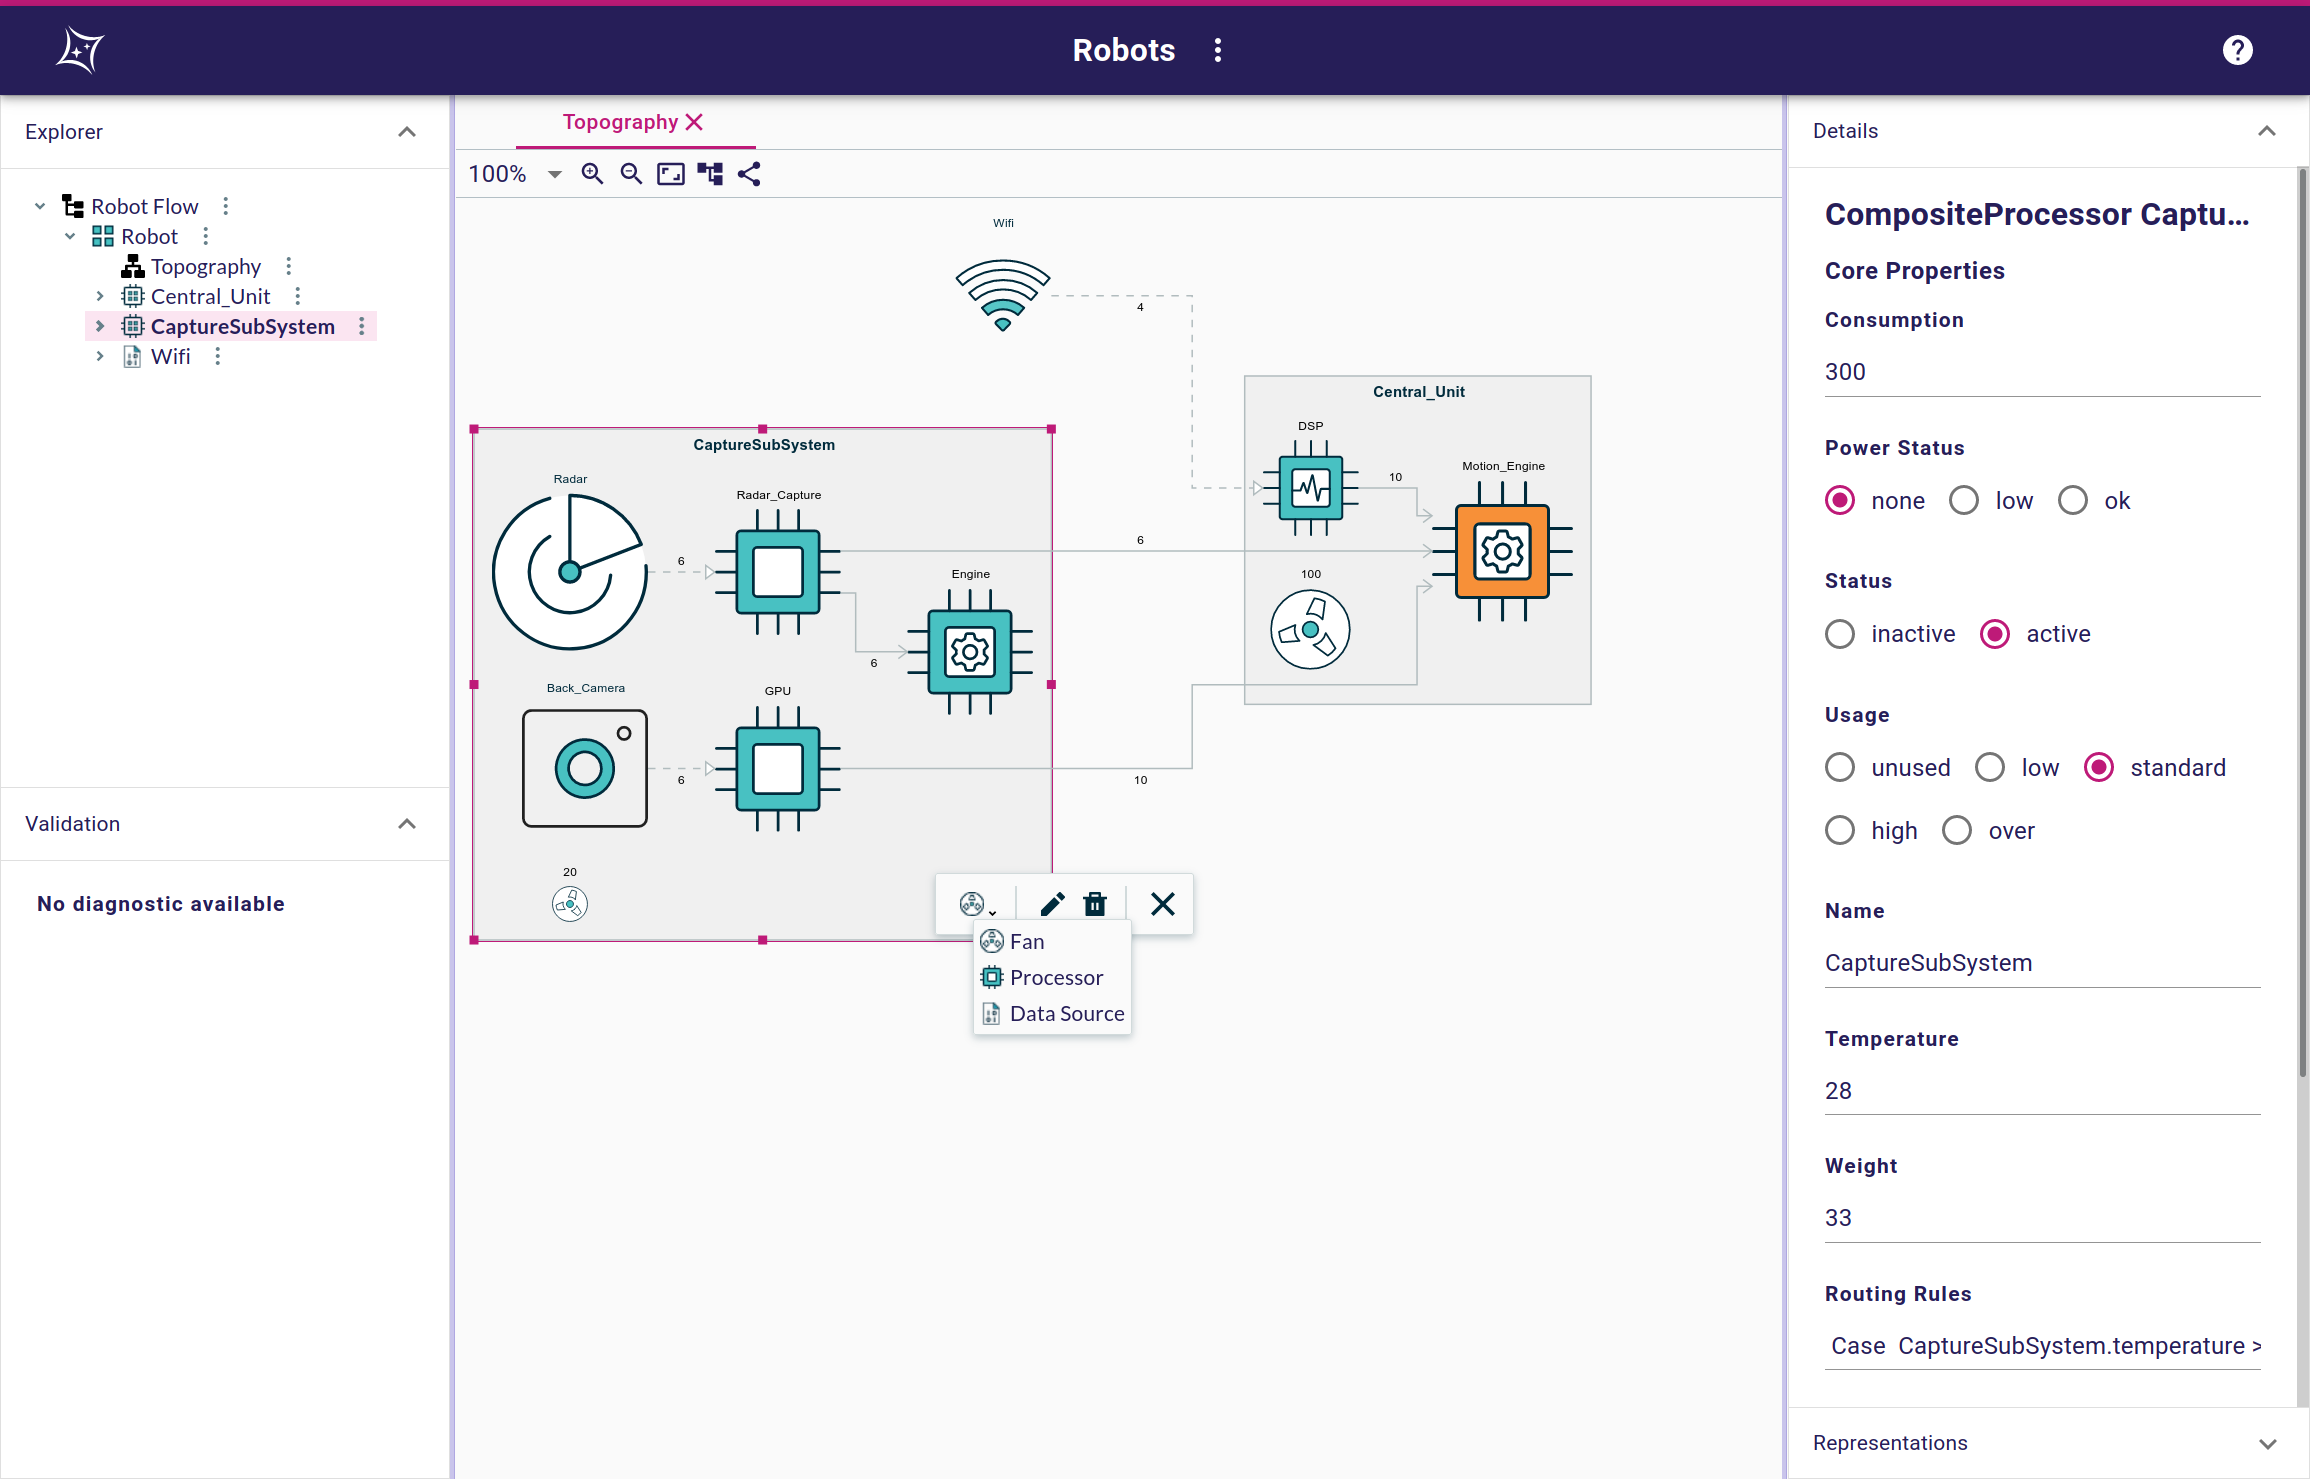
\includegraphics[width=0.95\linewidth]
	{./images/sirius-web-editor.png}
	\caption{Edytor modeli \SiriusWeb{}}\label{rys:sirius-web-ui}
	{\small Źródło: \url{https://github.com/eclipse-sirius/sirius-web}}
\end{figure}

% NOTE: manually move the first sentence to the next page to prevent a hanging
% sentence at the end of the page
\clearpage
\noindent \SiriusWeb{} składa się z 3 komponentów:
\begin{itemize}
	\item serwera aplikacyjnego stworzonego w technologii \emph{Java
		      Spring}~\cite{java-spring-homepage} dostarczającego
	      interfejsu sieciowego \emphgls{API} w formacie \GraphQL{}
	      pozwalającego na
	      wyświetlenie oraz modyfikację modelu,
	\item bazy danych \PostgreSQL{}~\cite{postgresql-homepage}
	      przechowującej informacje o modelach i użytkownikach,
	\item aplikacji przeglądarkowej napisanej z wykorzystaniem biblioteki
	      \React{}~\cite{react-homepage} umożliwiającej wyświetlenie i
	      modyfikację modeli
	      w formie drzewa obiektów lub diagramu.
\end{itemize}

Metamodele, na których bazuje \SiriusWeb{} są w tym samym formacie \Ecore{} co
metamodele w \SiriusDesktop{}. Można zatem w łatwy sposób stworzyć
graficzny edytor modeli zarówno w~formie aplikacji natywnej, jak i
przeglądarkowej. Posiadając istniejący metamodel języka użyty
w~\SiriusDesktop{} można go w krótkim czasie przenieść do \SiriusWeb{}. Jest
to~możliwe, ponieważ serwer aplikacyjny korzysta z tych samych bibliotek i
pakietów do obsługi metamodelu, które są wykorzystywane w edytorze
\SiriusDesktop{}.

Zmianie uległ natomiast sposób przechowywania modeli. W \SiriusDesktop{}
były one~zapisane w plikach na dysku użytkownika. W \SiriusWeb{} są one
przechowywane w bazie danych \PostgreSQL{}. Taki format zapisu pozwala na
równoczesny dostęp do modelu przez wielu użytkowników i natychmiastowe
przesyłanie informacji o zmianach w czasie rzeczywistym dzięki użyciu
\emph{GraphQL Subscriptions}~\cite{graphql-subscriptions} (dwukierunkowych
połączeń do przesyłania ustrukturyzowanych danych między przeglądarką a
serwerem opartych na protokole \WebSocket{}~\cite{wikipedia-websocket}).
Oznacza to, że użytkownicy mogą w czasie rzeczywistym wspólnie edytować modele
i~natychmiast widzieć zmiany wprowadzone przez innych użytkowników.
Poprzez zgrupowanie modeli w~projekty wewnątrz aplikacji \SiriusWeb{}
możliwa jest również kontrola dostępu do nich --- administrator może określić
zasady dostępu użytkowników do poszczególnych projektów.

Udostępnienie edytora modeli jako aplikacja przeglądarkowa sprawia też, że jest
on~bardziej dostępny dla użytkowników. Mogą oni przeglądać i edytować modele
bez instalacji aplikacji natywnych w ich systemie --- wystarczy przeglądarka
internetowa, która jest zainstalowana na większości komputerów konsumenckich.
Można też w łatwiejszy sposób podzielić się~przygotowanym przez nas modelem,
ponieważ wystarczy wysłać adres \emphgls{URL} innemu użytkownikowi zamiast
wysyłać plik z modelem.

Poza tym łatwiejsze wprowadzanie jest poprawek i zmian do metamodelu.
W przypadku aplikacji natywnych i dzieleniu się modelem przechowywanym w pliku
należało zaktualizować metamodel oraz wszystkie jego modele, a później wysłać
nowe pliki modeli oraz nowy edytor wszystkim użytkownikom. Problemy powstają
gdy użytkownicy zmodyfikowali swoje modele przechowywane lokalnie i nie są już
one kompatybilne z nowym metamodelem, lub gdy użytkownicy przypadkowo używają
starego modelu przy pracy z modelami. Takie rozwiązanie zwiększa liczbę
możliwości na popełnienie błędu. W przypadku aplikacji internetowej wszyscy
pracują z~tymi samymi modelami przechowywanymi na serwerze. Osoby
odpowiedzialne za~metamodel mogą go zmodyfikować wraz z modelami zapisanymi w
bazie danych. Uruchomienie serwera z~nowym metamodelem wystarcza, aby wszyscy
użytkownicy po~otworzeniu edytora \SiriusWeb{} mieli jego najnowszą
wersję.
